\documentclass[tikz,border=4pt]{standalone}
\usetikzlibrary{positioning}

\begin{document}
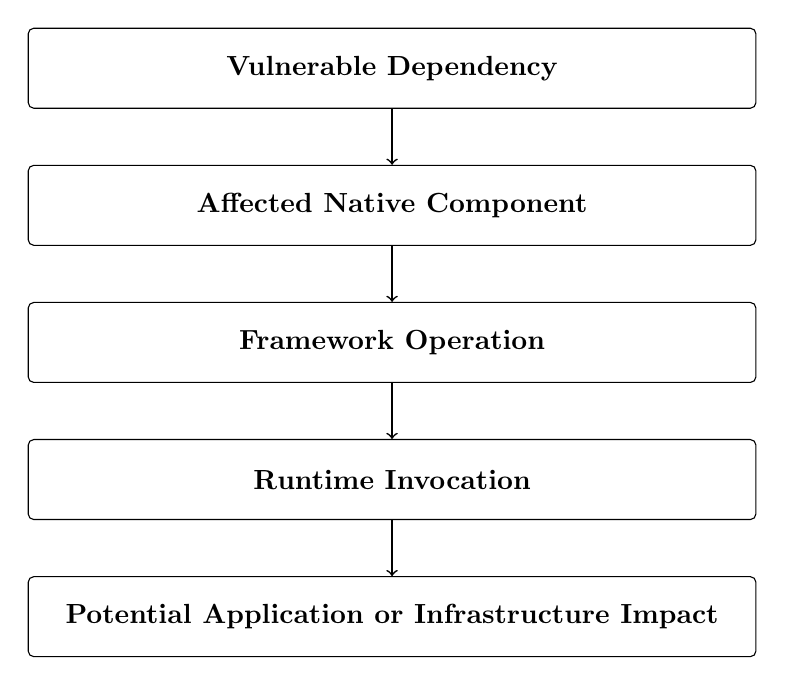
\begin{tikzpicture}[
  stage/.style={
    draw,
    rounded corners=2pt,
    text width=3.5in,
    minimum height=0.4in,
    align=center,
    font=\bfseries,
    inner sep=5pt
  },
  node distance=0.28in
]
\node[stage] (dependency) {Vulnerable Dependency};
\node[stage, below=of dependency] (native) {Affected Native Component};
\node[stage, below=of native] (framework) {Framework Operation};
\node[stage, below=of framework] (runtime) {Runtime Invocation};
\node[stage, below=of runtime] (impact) {Potential Application or Infrastructure Impact};

\draw[->, semithick] (dependency) -- (native);
\draw[->, semithick] (native) -- (framework);
\draw[->, semithick] (framework) -- (runtime);
\draw[->, semithick] (runtime) -- (impact);
\end{tikzpicture}
\end{document}
